\begin{question}
	Geef informeel de definitie van een lineair begrensde automaat (LBA). Argumenteer dat het aanvaardingsprobleem voor LBA's ($A_{LBA}$) beslisbaar is. Geef de stappen in een bewijs dat $E_{LBA}$ (de verzameling van LBA's die de lege taal bepalen) niet beslisbaar is.
\end{question}

\subsubsection*{Lineair begrensde automaat}

\begin{theorem}[Lineair Begrensde Automaat]
	Een Lineair Begrensde Automaat is een Turingmachine die niet leest of schrijft buiten het deel van de band dat initieel invoer bevat.
\end{theorem}

De naam komt hier tot stand door de volgende equivalente definitie van een lineair begrense automaat. Deze definitie laat toe dat de $LBA$ een stuk band gebruikt dat met een constante factor $f$ groter mag zijn dan de input.

\subsubsection*{$A_{LBA}$ is beslisbaar}

Het acceptatieprobleem voor $LBA$ is gedefinieerd als de taal
\begin{center}
	$A_{LBA} = \{<M,s>|M$ \textit{is een} $LBA$ \textit{en} $s \in L_{LBA}\}$
\end{center}

\begin{proof}
	We kijken naar alle mogelijke configuraties van een $LBA$ op een string van lengte $n$. Het aantal toestanden is $q$ met het aantal elementen in het bandalfabet $b$. Het aantal mogelijke strings is dan $b^n$. De leeskop kan onder elk van de symbolen staan terwijl de machine in elk van de toestanden kan zitten. Dat geeft in het totaal maximaal $qnb^b$ configuraties.
	We kunnen nu een beslisser $B$ voor $A_{LBA}$ construeren als volgt\footnote{Bij input $<M,s>$.}:
	\begin{enumerate}
		\item Berekent $k=qnb^n$.
		\item Simuleert dan $M$ op $s$ met maximaal $k$ stappen.
		\item Indien $M$ ondertussen accepteerde, accept.
		\item Indien $M$ ondertussen verwierp, reject.
		\item Indien $M$ nog niet stopte, betekent dat dat $M$ in een lus zit en dus niet zal accepteren: reject.
	\end{enumerate}
\end{proof}

\subsubsection*{$E_{LBA}$ is niet beslisbaar}

\begin{theorem}
	$E_{LBA} = \{M|M$ \textit{is een} $LBA$ \textit{die de lege taal bepaalt} $\}$ is niet beslisbaar. 
\end{theorem}

We laten eerst zien dat voor een gegeven Turingmachine $M$ en string $s$ we een $LBA$ kunnen construeren die gegeven een eindige rij configuraties (van $M$) kan beslissen of die rij een accepterende computation history is voor $s$. Een rij configuraties kan gemakkelijk op een band geplaatst worden zoals in de figuur hieronder.
	\begin{figure}[H]
  	\centering
    	  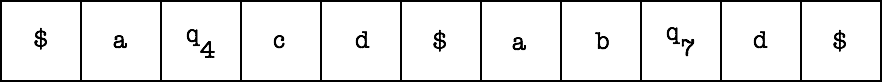
\includegraphics[width=0.8\textwidth]{./img/lba}
  	\caption{$\delta(q_4,c)=(q_7,b,R)$}
	\end{figure}
Wat moet de machine doen om na te gaan of een rij configuraties een accepterende computation history is voor $s$?
\begin{enumerate}
	\item Nakijken of twee opeenvolgende configuraties verbonden zijn door de $\delta$.
	\item Nakijken of de eerste configuratie $q_s$ bevat op de juiste plaats.
	\item NAkijken of de laatste configuratie $q_a$ bevat.
\end{enumerate}
Zonder veel in detail te treden moet het duidelijk zijn dat hiervoor slechts een constante hoeveelheid extra bandruimte nodig is en dat die beslissing dus kan  genomen worden door een $LBA$. We maken die $LBA$ zo dat hij bij een accepterende computation history accepteert en anders reject. Nu kunnen we aan het bewijs zelf beginnen.

\begin{proof}
	Stel dat we een beslisser $E$ hebben voor $E_{LBA}$. We construeren een beslisser $B$ voor $A_{TM}$ als volgt. Bij input $<M,s>$ doet $B$:
	\begin{enumerate}
		\item Construeer de $LBA$ $A_{M,s}$ die van input kan beslissen of een inputstring een accepterende computation history is voor $M$ op input $s$.
		\item Laat $E$ los op $<A_{M,s}>$: als $E$ aanvaardt, reject; anders accept.
	\end{enumerate}
	\begin{center}
		$B$ beslist $A_{TM}$ want $B$ accepteert $<M,s>$\\
		$\Updownarrow$\\
		$E$ $<A_{M,s}>$ reject\\
		$\Updownarrow$\\
		$A_{M,s}$ aanvaardt minstens \'e\'en string\\
		$\Updownarrow$\\
		Er bestaat een accepterende computation history voor $M$ op $s$
	\end{center}
	Het laatste is equivalent met zeggen dat $M$ $s$ accepteert.
	Die $B$ kan niet bestaan, dus ook $E$ niet en $E_{LBA}$ is onbeslisbaar.
\end{proof}